% ----------------------------------------------------------------
% Article Class (This is a LaTeX2e document)  ********************
% ----------------------------------------------------------------
\documentclass{article}
\usepackage[english]{babel}
\usepackage{styfiles/proof, styfiles/code, amsmath,amsthm}
\usepackage{amssymb}  % for "\leadsto"
\usepackage{bbold}%for typeface: mathbb
\usepackage{graphicx} %to insert pic from file
\usepackage{hyperref}
% THEOREMS -------------------------------------------------------
\newtheorem{thm}{Theorem}[section]
\newtheorem{cor}[thm]{Corollary}
\newtheorem{lem}[thm]{Lemma}
\newtheorem{prop}[thm]{Proposition}
\theoremstyle{definition}
\newtheorem{defn}[thm]{Definition}
\theoremstyle{remark}
\newtheorem{rem}[thm]{Remark}
\numberwithin{equation}{section}

% ----------------------------------------------------------------
\begin{document}

\newcommand{\env}[1]{[\![#1]\!]\kappa}
\newcommand{\round}[1]{(\!|#1|\!)}

\title{Hoisting, Allocation and Code Generation}%
\author{Di Zhao}%
%\address{address}%
%\thanks{}%\sqrt{}
\date{\small{\texttt{zhaodi01@mail.ustc.edu.cn}}}%
% ----------------------------------------------------------------

\maketitle
% ----------------------------------------------------------------

Document for the hoisting and allocation phases.

\section{Hoisting}

Hoist all the function definitions
to top-level. Source language : closure passing language.

\begin{figure}[!ht]
  % Requires \usepackage{graphicx}
  \centering
\begin{tabular}{rrcl}
(terms) & $K$ & $\to$ & \textsf{letval }$x\ =\ V$ \textsf{ in } $K$ \\
        &     & $|$ & \textsf{let }$x = \texttt{\#}i\ y$\textsf{ in }$K$\\
        &     & $|$ & \textsf{letcont }$k\ env\ x = K$\textsf{ in }$K'$\\
        &     & $|$ &  $k\ env\ x$ \\
        &     & $|$ & $f\ env\ k\ x$ \\
        &     & $|$ & \textsf{case} $x$ \textsf{of}
             $\overrightarrow{\textsf{in}i_j\ x_j \Rightarrow K_j}$\\
        &     & $|$ & \textsf{letprim} $x=PrimOp\ \vec{y}
         \textsf{ in}\ K$\\
        &     & $|$ &\textsf{if} $x$ \textsf{then} $K\ \textsf{else}\ K'$\\
        &     & $|$ &\textsf{letfix }$f\ env\ k\ x=K$\textsf{ in }$K'$\\

(values) & $V$ & $\to$ & () \\
        &     & $|$ & \texttt{true}\\
        &     & $|$ & \texttt{false}\\
        &     & $|$ & $i$\\
        &     & $|$ & $"s"$\\
        &     & $|$ & ($x_1,x_2,\ ...\ , x_n$)\\
        &     & $|$ & \texttt{in}$i\ x$\\
        &     & $|$ &  $\lambda env\ k\ x.K$ \\

(primitive & $PrimOp$ & $\to$ & $+\ $ $|\ -\ |$ $\ *$\\
operations) &     & $|$ & $>\ |\ <\ |\ =$\\
        &     & $|$ & $\textsf{andalso }\ |\ \textsf{ orelse }\ |\ \textsf{ not}$\\
        &     & $|$ & \textsf{print} $|$ \textsf{int2string}\\
\end{tabular}
  \caption{Closure syntax}
  \label{fig-sub}
\end{figure}

The target language in this section is called Flat. The syntax is shown in Figure 2.

\begin{figure}[!ht]
  % Requires \usepackage{graphicx}
  \centering
\begin{tabular}{rrcl}
       &     &  &\\
(program) & $p$ & $\to$ & $m$; $\vec{f}$ \\

(functions) & $m,\ f$ & $\to$ & $x$ $\vec{y}$ \{
      $\vec{b};$  $\ e$; \}\\

(bindings) & $b$ & $\to$ & $x=v$ \\

(values) & $v$ & $\to$ & () \\
        &     & $|$ & \texttt{true}\\
        &     & $|$ & \texttt{false}\\
        &     & $|$ & $i$\\
        &     & $|$ & $"s"$\\
        &     & $|$ & $\pi _i\ x$\\
        &     & $|$ & ($x_1,x_2,\ ...\ , x_n$)\\
        &     & $|$ & \textsf{in}$_i\ x$\\
        &     & $|$ &  $PrimOp\ \vec{x}$\\

(primitive & $PrimOp$ & $\to$ & $+\ $ $|\ -\ |$ $\ *$\\
operations) &     & $|$ & $>\ |\ <\ |\ =$\\
        &     & $|$ & $\textsf{andalso }\ |\ \textsf{ orelse }\ |\ \textsf{ not}$\\
        &     & $|$ & \textsf{print} $|$ \textsf{int2string}\\

(transfers) & $e$ & $\to$ & $x$ $\vec{y}$\\
        &     & $|$ & \texttt{if} $x$ \texttt{then} $e_1$ \texttt{else} $e_2$\\
        &     & $|$ & \textsf{case} $x$ \textsf{of}
         $\overrightarrow{\textsf{in}i_j\ x_j \Rightarrow e_j}$\\
       % &     & $|$ & \textsf{exit} $x$
\end{tabular}
  \caption{Flat syntax}
  \label{fig-sub}
\end{figure}

In the Flag language, a program $p$ consists of a main function
(denoted as $m$) and a list of functions ($\vec{f}$).

In a function definition $x$ $\vec{y}$ \{ $\vec{b};$  $\ e$; \},
$x$ is the function name, $\vec{y}$ is the list of arguments.
 The function body consists of a list of
 bindings $\vec{b}$ and one control transferring expression $e$.

A binding binds a value $v$ to a name $x$. Here the
values to be named include empty value, constant integers, constant strings,
projection operation, tuples, tagged values and primary operations.

There're three kinds of control transferring expressions (denoted as $e$).

The hoisting rules are illustrated in Figure 3.

\begin{figure}[!ht]
  % Requires \usepackage{graphicx}
  \centering
\begin{tabular}{c}
$$\infer[(\textsc{H-LetValFunc})]
        {\vdash\textsf{letval }x=\lambda env\ k\ z.K\textsf{ in }K'
            \leadsto (\vec{f_1}::\vec{f_2},::f_x,\ \vec{b_2},\ e_2)}
        {\vdash K \leadsto (\vec{f_1},\vec{b_1}, e_1) \ \
            \vdash K' \leadsto (\vec{f_2},\vec{b_2}, e_2)}$$\\
    where $f_x$ is function: $x\ [env,k,z]\{\vec{b_1};\ e_1;\}$ \\\\
                                                                 % LetValFunc
$$\infer[(\textsc{H-LetVal})]
        {\vdash\textsf{letval }x=V\textsf{ in }K
            \leadsto (\vec{f},(x=V)::\vec{b}, e)}
        {\vdash K \leadsto (\vec{f},\vec{b}, e)}$$\\\\
                                                                 % LetVal
$$\infer[(\textsc{H-Let})]
        {\vdash\textsf{let }x=\pi_i\ y\textsf{ in }K
            \leadsto (\vec{f},(x=\pi_i\ y)::\vec{b}, e)}
        {\vdash K \leadsto (\vec{f},\vec{b}, e)}$$\\\\
                                                                 % Let
$$\infer[(\textsc{H-LetCont})]
        {\vdash\textsf{lecont }k\ env\ x=K\textsf{ in }K'
            \leadsto (\vec{f_1}::\vec{f_2},::f_k,\ \vec{b_2},\ e_2)}
        {\vdash K \leadsto (\vec{f_1},\vec{b_1}, e_1) \ \
            \vdash K' \leadsto (\vec{f_2},\vec{b_2}, e_2)}$$\\
    where $f_k$ is function: $k\ [env,x]\{\vec{b_1};\ e_1;\}$ \\\\
                                                                 % LetCont
$$\infer[(\textsc{H-ContApp})]{\vdash k\ env\ x\leadsto ([\ ],[\ ], k\ [env, x])}{}$$\\\\
                                                                 % ContApp
$$\infer[(\textsc{H-FuncApp})]{\vdash f\ env\ k\ x\leadsto ([\ ],[\ ], f\ [env,k,x])}{}$$\\\\
                                                                 % FuncApp
$$\infer[(\textsc{H-Case})]
        {\vdash \textsf{case}\ x\ \textsf{of}
         \ \overrightarrow{\textsf{in}i_j\ x_j \Rightarrow K_j}
            \leadsto (\vec{f_1}::...::\vec{f_n}
                ,\ \vec{b_1}::...::\vec{b_n}
                ,\ \textsf{case}\ x\ \textsf{of}
                \ \overrightarrow{\textsf{in}i_j\ x_j \Rightarrow e_j})}
        {\vdash K_j \leadsto (\vec{f_j},\vec{b_j}, e_j)}$$\\
            where $j=1,\ ...\ , n$\\\\
                                                                 % Case
$$\infer[(\textsc{H-LetPrim})]
        {\vdash\textsf{letprim}\ x=PrimOp\ \vec{y} \texttt{ in}\ K
           \leadsto (\vec{f},(x, PrimOp\ \vec{y})::\vec{b}, e)}
        {\vdash K \leadsto (\vec{f},\vec{b}, e)}$$\\\\
                                                                 % LetPrim
$$\infer[(\textsc{H-If})]
        {\vdash \textsf{if } x \textsf{ then } K\ \textsf{else}\ K'
            \leadsto }
        {\vdash K \leadsto (\vec{f_1},\vec{b_1}, e_1) \ \
            \vdash K' \leadsto (\vec{f_2},\vec{b_2}, e_2)}$$\\
            $(\vec{f_1}::\vec{f_2}
                ,\ \vec{b_1}::\vec{b_2}$,
                \ \texttt{if} $x$ \texttt{then} $e_1$ \texttt{else} $e_2$)\\\\
                                                                 % If
$$\infer[(\textsc{H-LetFix})]
        {\vdash\textsf{letfix }f\ env\ k\ x=K\textsf{ in }K'
            \leadsto (\vec{f_1}::\vec{f_2},::f_f,\ \vec{b_2},\ e_2)}
        {\vdash K \leadsto (\vec{f_1},\vec{b_1}, e_1) \ \
            \vdash K' \leadsto (\vec{f_2},\ \vec{b_2},\ e_2)}$$\\
    where $f_f$ is function: $f\ [env,k,x]\{\vec{b_1};\ e_1;\}$ \\
                                                                 % LetFix
\end{tabular}
  \caption{Hoisting rules for Closure.t}
  \label{fig-sub}
\end{figure}

$\ $\\

\noindent{
Updates:
\begin{description}
  \item[15-7-3:]
  Change the form of \texttt{case} in \texttt{flat.sig}, \texttt{flat.sml},
  and changed the respective hoisting rule in \texttt{hoist.sml}
  to enable multiple cases .
  
  \item[15-9-5:]
  Added boolean values and corresponding operations. Changed \texttt{if0}
  expression into \texttt{if} expression.
\end{description}
}

\section{Allocation}

After the allocation
 process, the allocation and initialization of tuples and tagged values will
be explicit. Besides, the arguments of a single function are packed into
one single argument, so that it would be easier to scan over the arguments
 when performing garbage collection. The target language in this phase is called:
 Machine. The syntax of Machine language is shown in Figure 4.

\begin{figure}[!ht]
  % Requires \usepackage{graphicx}
  \centering
\begin{tabular}{rrcl}
(program) & $P$ & $\to$ & $m$; $\vec{f}$ \\

(functions) & $m,\ f$ & $\to$ & $x$ $y$ \{
      $\overrightarrow{binding};$  $\ b$; \}\\

(bindings) & $binding$ & $\to$ & $x=v$ \\
        &     & $|$ & $dst\texttt{[}i\texttt{]}=src$\\

(values) & $v$ & $\to$ & \texttt{null} \\
        &     & $|$ & \texttt{true}\\
        &     & $|$ & \texttt{false}\\
        &     & $|$ & $i$\\
        &     & $|$ & $"s"$\\
        &     & $|$ & $x\texttt{[}i\texttt{]}$\\
        &     & $|$ & \texttt{allocTuple}($i$)\\
        &     & $|$ & \texttt{allocTag}($i$)\\
        &     & $|$ &  $PrimOp\ \vec{x}$\\

(primitive & $PrimOp$ & $\to$ & $+\ $ $|\ -\ |$ $\ *$\\
operations) &     & $|$ & $>\ |\ <\ |\ =$\\
        &     & $|$ & $\textsf{andalso }\ |\ \textsf{ orelse }\ |\ \textsf{ not}$\\
        &     & $|$ & \textsf{print} $|$ \textsf{int2string}\\

(blocks) & $b$ & $\to$ &  $\overrightarrow{binding};$  $\ e$\\

(transfers) & $e$ & $\to$ &  $x$ $y$\\
        &     & $|$ & \texttt{if} $x$ \texttt{then} $b_1$ \texttt{else} $b_2$\\
        &     & $|$ & \textsf{case} $x$ \textsf{of}
         $\overrightarrow{\textsf{in}i_j\ x_j \Rightarrow b_j}$\\
\end{tabular}
  \caption{Machine syntax}
  \label{fig-sub}
\end{figure}

Given the Machine syntax, we can decide the conversion rules intuitively, as
shown in Figure 5, 6, 7.

\begin{figure}[!ht]
  % Requires \usepackage{graphicx}
  \centering
\begin{align*}
\mathcal{A}_b : \textrm{string * Flat.binding} &\to \textrm{Machine.binding list}\\ %header
\mathcal{A}_b(x=()) & = [x=\texttt{null}]\\ %empty
\mathcal{A}_b(x=\texttt{true}) & = [x=\texttt{true}]\\ %true
\mathcal{A}_b(x=\texttt{false}) & = [x=\texttt{false}]\\ %false
\mathcal{A}_b(x=i) & = [x=i]\\ %number
\mathcal{A}_b(x="s") & = [x="s"]\\ %string
\mathcal{A}_b(x=\pi _i\ y) & = [x=y\texttt{[}i\texttt{]}]\\ %proj
\mathcal{A}_b(x=(x_1,x_2,\ ...\ , x_n)) & = [x=\texttt{allocTuple}(n),\\
    &\kern0.5cm x\texttt{[}1\texttt{]}=x_1,\\
    &\kern0.5cm...\\
    &\kern0.5cm x\texttt{[}n\texttt{]}=x_n]\\ %tuple
\mathcal{A}_b(x=\textsf{in}_i\ y) & = [x=\texttt{allocTag}(i),\\
    &\kern0.5cm x\texttt{[}1\texttt{]}=y]\\ %tag
\mathcal{A}_b(x=PrimOp\ \vec{y}) & = [x=PrimOp\ \vec{y}] %primop
\end{align*}
  \caption{Conversion from Flat to Machine for bindings}
  \label{fig-sub}
\end{figure}

\begin{figure}[!ht]
  % Requires \usepackage{graphicx}
  \centering
\begin{align*}
\mathcal{A}_e : \textrm{Flat.e} &\to \textrm{Machine.block}\\ %header
\mathcal{A}_e(x\ \vec{y}) & = [z=\texttt{allocTuple}(n),\\
    & \kern0.5cm z\texttt{[}1\texttt{]}=y_1,\\
    & \kern0.5cm ...\\
    & \kern0.5cm z\texttt{[}n\texttt{]}=y_n];\\
    & \kern0.5cm x\ z \\%call
    &(\textrm{given that}\ \vec{y}=[y_1,\ ...\ , y_n])\\
\mathcal{A}_e(\texttt{if}\ x\ \texttt{then}\ e_1\ \texttt{else}\ e_2) & = [\ ];\\
    & \kern0.5cm \texttt{if}\ x\ \texttt{then}\ \mathcal{A}_e(e_1)
        \ \texttt{else}\ \mathcal{A}_e(e_2) \\   %if
\mathcal{A}_e(\textsf{case}\ x\ \textsf{of}
         \ \overrightarrow{\textsf{in}i_j\ x_j \Rightarrow e_j})
    & = [\ ];\\
    & \kern0.5cm \textsf{case}\ x\ \textsf{of}
         \ \overrightarrow{\textsf{in}i_j\ x_j \Rightarrow \mathcal{A}_e(e_j)}   %case
\end{align*}
  \caption{Conversion from Flat to Machine for expressions}
  \label{fig-sub}
\end{figure}

\begin{figure}[!ht]
  % Requires \usepackage{graphicx}
  \centering
\begin{align*}
\mathcal{A}_f(x\ \vec{y}\ \{\ \vec{b};\ e; \})
    &= x\ (z)\ \{\\
    &\kern1cm \overrightarrow{y_i=z[i]}::\\
    &\kern1cm \overrightarrow{\mathcal{A}_b(b)};\\
    &\kern1cm \mathcal{A}_e(e); \\
    &\kern0.4cm \}\\
    (\textrm{given that}&\ \vec{y}=[y_1,\ ...\ , y_n],\ i =1,\ ...\ ,n)
\end{align*}
  \caption{Conversion from Flat to Machine for functions}
  \label{fig-sub}
\end{figure}

As for bindings, because tuples and tagged values are structured data elements,
we need to allocate space for them and perform some initializations. In this way,
both of them require special treatment:
\begin{itemize}
  \item For $x=(x_1, ..., x_n)$, allocate a tuple $x$ with $n$ components and initialize
    component $x\texttt{[}i\texttt{]}$ with $x_i$.
  \item For $x=in_i\ y$, allocate structure $x$ with tag value $i$ and initialize
    component $x\texttt{[}1\texttt{]}$ with $y$.
\end{itemize}

Arguments of a function call now need to be packed
into a tuple, and the tuple needs to be initialized by these arguments. In this way,
 control transferring expressions will be translated into a \textit{block} which
 consists of a list of bindings and an expression.

For the same reason above, in a function definition, the original arguments
need to be fetched out from the sole parameter of the function. Namely we
need to add some bindings ahead of the original function body.

Pay attention that as the main function $m$ takes no arguments, no additional
bindings for argument folding is needed.

$\ $\\

\noindent{
Updates:
\begin{description}
  \item[15-7-4:]
  Change the form of \texttt{case} in \texttt{machine.sig}, \texttt{machine.sml},
  and changed the respective allocation rule in \texttt{codegen.sml}
  to enable multiple cases .
  
  \item[15-9-5:]
  Added boolean values and corresponding operations. Changed \texttt{if0}
  expression into \texttt{if} expression.
\end{description}
}

\section{Code Generation}

Code generation procedure: encode the functions to output the
Machine syntax tree into a \texttt{.c} file which can be compiled by
a C compiler and then be executed.

As is shown Figure 4, the Machine syntax is basically C style syntax.
Consequently we can output C code for most of the syntax terms directly without making
much modifications. However, there are a few aspects to which you may pay attention:

\begin{itemize}
  \item Type and type-casting. As C is strong typed, you'll have to declare
  variables and insert type-castings with explicit types. For example, you can
  declare all the variables with \texttt{int*} type; when performing a
  function call, you may cast the function name into \texttt{void * (*)()} type first.
  \item Bindings of tuples and tagged values are encoded as function calls to
  \texttt{allocTuple} and \texttt{allocTag} respectively. You'll need to implement
  these two functions in the runtime system.
  \item A case expression: $\textsf{case}\ x\ \textsf{of}
         \ \overrightarrow{\textsf{in}i_j\ x_j \Rightarrow b_j}$ can be encoded as an
  switch structure. The variables
  $x_j$ should be initialized (by what value?) before the switch structure.
\end{itemize}

To support the output code, we need to provide a runtime system, including the definition
 of function \texttt{allocTuple} and \texttt{allocTag}. Therefore, we need to decide
the memory map for these structures.

As we rely on garbage
collection to retrieve memory space, some additional information needs to be attached,
 such as the length of a tuple, or to distinguish between integers, tuples and tagged
 values. We will discuss about this with more details in
the next lab. For now we just use a simple strategy shown in Figure 8 and 9.

\begin{figure}
  \centering
  % Requires \usepackage{graphicx}
  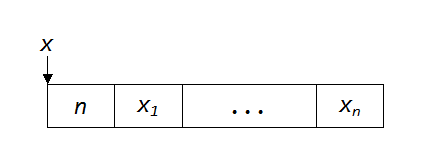
\includegraphics[width=0.5\textwidth]{tuple.png}\\
  \caption{memory map for tuple $x=(x_1,\ ...,\ x_n)$}\label{fig:digit}
\end{figure}

\begin{figure}
  \centering
  % Requires \usepackage{graphicx}
  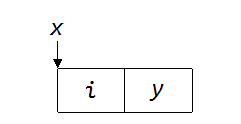
\includegraphics[width=0.28\textwidth]{tag.png}\\
  \caption{memory map for tagged value $x=\textsf{in}_i\ y$}\label{fig:digit}
\end{figure}

As is shown in Figure 8, a tuple with $n$ components will occupy $n+1$ memory
cells. The first cell is to store the length of the tuple, the rest $n$ cells
store the component values in order. In this lab, each cell is constraint to be 4 Bytes.
In this way, \texttt{allocTuple(n)} will allocate a memory space of $4*(n+1)$ Bytes
and store the value $n$ in the first cell. Finally it returns a pointer to
the first cell. The value of the components will be loaded later via this
pointer.

Note that we will never visit a tuple with the length of 0, so we can simply
output "\texttt{x=0}" instead of "\texttt{x=allocTuple(0)}".

As shown in Figure 9, a tagged value $\textsf{in}_i\ y$ takes two memory
cells. The first cell is to store the tag value $i$ (1 or 2), while the second
one for the value to be tagged.
In this way, \texttt{allocTag(i)} will allocate a memory space of 8kb
and store the tag value $i$ in the first cell. And finally it will return a pointer to
the first cell. The value $y$ will be loaded later via this pointer.\\



\end{document}
